
%%%%%%%%%%%%%%%%%%%%%%%%%%%%%%%%%%%%%%%%%%%%%%%%%%%%%%%%%%%%%%%%%%%%%%%%%%%%%%
%%% Preamble

%%% Document Type
\documentclass[11pt,openany]{memoir} % 'openany': allows chapters to open on left and right pages; avoids blank pages between chapters to force opening on right
\chapterstyle{section}

%%% Packages
\usepackage{amsmath,amssymb,cancel,units} % math environment and symbols
\usepackage{array}                        % for better arrays (eg matrices) in maths
\usepackage{paralist}                     % very flexible & customisable lists (eg. enumerate/itemize, etc.)
\usepackage{verbatim}                     % adds environment for commenting out blocks of text & for better verbatim
\usepackage[pdftex,bookmarks,colorlinks,breaklinks]{hyperref}  % PDF hyperlinks, with coloured links
\usepackage{memhfixc}                     % remove conflict between the memoir class & hyperref
\usepackage{graphicx}                     % Add graphics capabilities
\usepackage{xspace}                        % smart space insertion after commands
\usepackage{tabulary}
\usepackage[table]{xcolor} % http://tex.stackexchange.com/questions/5363/how-to-create-alternating-rows-in-a-table
\usepackage{wrapfig}

%% Following allows for bulleted definition lists ('description' environment)
%% by declaring \SpecialItem before the list;
%% from: http://tex.stackexchange.com/questions/57876/add-bullet-points-to-description-lists
\let\Item\item
\newcommand\SpecialItem{\renewcommand\item[1][]{\Item[\textbullet~\bfseries##1]}}
\renewcommand\enddescription{\endlist\global\let\item\Item}


\usepackage{listings}
\definecolor{mygreen}{rgb}{0,0.6,0}
\definecolor{mygray}{rgb}{0.5,0.5,0.5}
\definecolor{mymauve}{rgb}{0.58,0,0.82}

\lstset{ %
  backgroundcolor=\color{white},            % choose the background color; you must add \usepackage{color} or \usepackage{xcolor}
  basicstyle=\footnotesize\ttfamily,        % the size of the fonts that are used for the code
  breakatwhitespace=false,                  % sets if automatic breaks should only happen at whitespace
  breaklines=true,                          % sets automatic line breaking
  captionpos=b,                             % sets the caption-position to bottom
  commentstyle=\color{mygreen},             % comment style
  deletekeywords={...},                     % if you want to delete keywords from the given language
  escapeinside={\%*}{*)},                   % if you want to add LaTeX within your code
  extendedchars=true,                       % lets you use non-ASCII characters; for 8-bits encodings only, does not work with UTF-8
  frame=single,	                            % adds a frame around the code
  columns=fullflexible,
  keepspaces=true,                          % keeps spaces in text, useful for keeping indentation of code (possibly needs columns=flexible)
  keywordstyle=\color{blue},                % keyword style
  % language=Octave,                          % the language of the code
  otherkeywords={*,...},                    % if you want to add more keywords to the set
  % numbers=left,                             % where to put the line-numbers; possible values are (none, left, right)
  % numbersep=5pt,                            % how far the line-numbers are from the code
  % numberstyle=\tiny\color{mygray},        % the style that is used for the line-numbers
  rulecolor=\color{black},                  % if not set, the frame-color may be changed on line-breaks within not-black text (e.g. comments (green here))
  showspaces=false,                         % show spaces everywhere adding particular underscores; it overrides 'showstringspaces'
  showstringspaces=false,                   % underline spaces within strings only
  showtabs=false,                           % show tabs within strings adding particular underscores
  stepnumber=2,                             % the step between two line-numbers. If it's 1, each line will be numbered
  stringstyle=\color{mymauve},              % string literal style
  tabsize=2,	                            % sets default tabsize to 2 spaces
  title=\lstname                            % show the filename of files included with \lstinputlisting; also try caption instead of title
}

%%% Notation and Variables

\newcommand{\targetData}{D}
\newcommand{\trainingDataForModel}[1]{D^{*#1}}
\newcommand{\trainingDataSet}{\mathbf{D}^{*}}
\newcommand{\summaryStatisticFunction}{S}
\newcommand{\modelCategory}[1]{M_{#1}}
\newcommand{\modelCategories}{\mathbf{M}}

%%%%%%%%%%%%%%%%%%%%%%%%%%%%%%%%%%%%%%%%%%%%%%%%%%%%%%%%%%%%%%%%%%%%%%%%%%%%%%%
%% Main Document
\begin{document}
% \rowcolors{2}{gray!25}{gray!15}

\title{ARCHIPELAGO}
\author{Jeet Sukumaran}
\maketitle
\setsecnumdepth{subsubsection}

\chapter{Introduction}

``Archipelago'' is the name of a generative phylogeny-based model that simultaneously incorporates the diversification processes of speciation and extinction nad the biogeographical processes of area gain (``dispersal'') and area loss (``extirpation''), with these processes being differentially regulated by ecological or other traits that are themselves co-evolving on the phylogeny.
The theory and background to this model and its usage is described in the following paper:


This software project, ``archipelago'' presents a suite of programs to generate and analyze data under the Archipelago model.
The primary objective of the analysis is \textit{model selection}: i.e., statistically identifying the model that generated a particular set of data.
% to \textit{classify a dataset with respect to the model that generated it}.
``archipelago'' is, thus, a computational biogeographical model selection analysis package that exploits the power and flexibility of the Archipelago model to allow you to ask and answer historical biogeographical questions of a nature and complexity that are not possible under any other approach.
In particular, instead of asking questions about ancestral area patterns, you can ask questions about processes, and how some processes (e.g., ecology) affect other processes (e.g., dispersal or speciation).

\chapter{Installation}

\section{Pre-requisites}

\begin{itemize}
    \item Python 2.7 or higher
    \item DendroPy Phylogenetic Computing Library, version 4 or above (\url{http://dendropy.org}).
    \item R (\url{http://www.r-project.org/})
    \item The following R packages:
    \begin{itemize}
        \item adegenet
        \item picante
        \item BioGeoBears
        \item GEIGER
    \end{itemize}
\end{itemize}

\section{Installation from Source}

Run the following in the top-level directory of the project:

\begin{lstlisting}
    python setup.py install
\end{lstlisting}


\chapter{Usage}

\section{Overview of Workflow}

\begin{figure}[h!]
    \begin{center}
        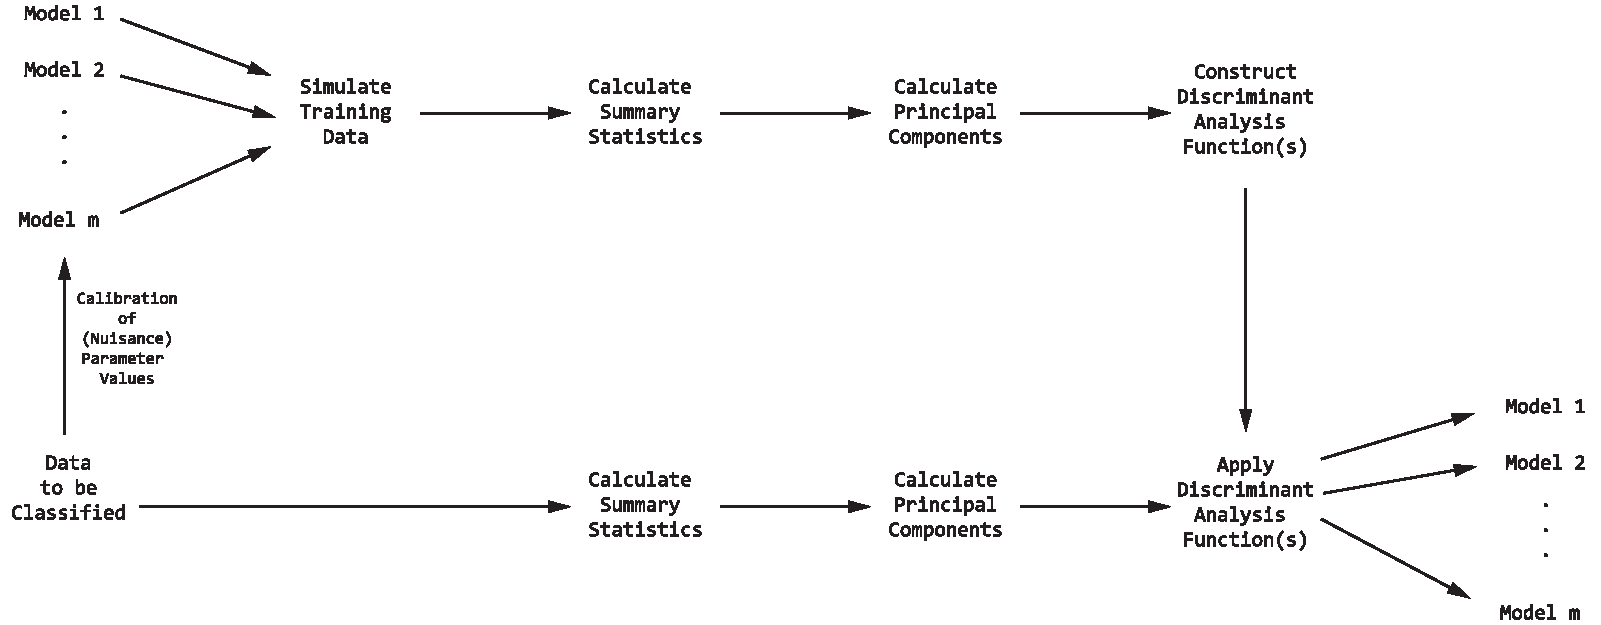
\includegraphics[scale=0.5]{figs/flowchart1.pdf}
        % \caption{default}
        % \label{fig:default}
    \end{center}
\end{figure}

Let $\targetData$ be the \textit{target} data, consisting of an ultrametric phylogeny with each of the tips associated with a geographic range (presence/absence over one or more areas) as well as with set of trait states.
Let $\modelCategories = \{\modelCategory{1}, \modelCategory{2}, ... \modelCategory{m}\}$ be a set of $k$ models that we are interested in studying.
Let $\summaryStatisticFunction(\cdot)$ be a function that takes a set of data returns a set of summary statistics.
Our analytical objective is, for each $\modelCategory{i}, \modelCategory{i} \in \modelCategories$, estimate the probability that it generated the target data $\targetData$, relative to all the other models in $\modelCategories$.
The operational procedure consists of the following steps:
\begin{enumerate}
    \item \textbf{Simulation of Training Data}: For each $\modelCategory{i}, \modelCategory{i} \in \modelCategories$, simulate $n$ replicates of data, $\trainingDataForModel{i}$. We label each replicate of this data with the name of the model that generated it (e.g., ``Model $i$''). The set of all data so generated constitutes the training data, $\trainingDataSet$.
    \item \textbf{Calculation of Summary Statistics}: Calculate summary statistics on the training data to yield, $\summaryStatisticFunction(\trainingDataSet)$, and summary statistics on the target data to yield $\summaryStatisticFunction(\targetData)$.
    \item \textbf{Classification of Target Data}: Construct a Discriminant Analysis (DA) function on principal components (PC) calculated on the training data set summary statistics, $\summaryStatisticFunction(\trainingDataSet)$; apply the discriminant analysis function to principal components calculated on the summary statistics of the target data, $\summaryStatisticFunction(\targetData)$.
\end{enumerate}

\section{Simulation of Training Data}

We use the program, ``\texttt{archipelago-simulate.py}'', to simulate the data under each model in the set of competing models.
The simulation program is run separately for each of the models, with multiple independent replicates in each run.
Full details on this program invocation can be found by running:
\begin{lstlisting}
    archipelago-simulate.py --help
\end{lstlisting}
A typical invocation of the program will have the following arguments:
\begin{description}
    \SpecialItem
    \item[``MODEL-FILE''] \hfill \\
        A JSON or Python file containing nothing but a dictionary specifying the full model under which to simulate data. This is described in detail in the \hyperref[sec:model-specification]{Model Specification} section.
    \item[``\texttt{-n}'' or ``\texttt{--nreps}''] \hfill \\
        The number of independent replicates to simulate under this model.
    \item[``\texttt{-o}'' or ``\texttt{--output-prefix}''] \hfill \\
        The path and filename stem where the results will be saved.
\end{description}
For example,
\begin{lstlisting}
    archipelago-simulate.py -n 100 -o results/m1 model1.json
\end{lstlisting}
will run 100 replicates under the model specified in the file ``model1.json'' and all output will saved to files in the ``results/'' subdirectory with filenames beginning with ``m1''.

The simulation program produces the following output:
\begin{description}
    \SpecialItem
        \item[\texttt{<OUTPUT-PREFIX>.focal-areas.trees}] \hfill \\
            A collection of phylogenies in NEWICK format, where each phylogeny represents the result from a single simulation replicate.
            The tips of these trees represent lineages that occur in at least one of the focal areas (in contrast to the phylogenies in the ``\texttt{all-areas.trees}'' file, where \textit{all} extant lineages are represented, regardless of where they occur).
            The distribution and trait states of the tip lineages are encoded in the tip labels.
            This is the data that is of primary analytical interest, and will be passed to the summary statistics calculation program, \texttt{archipelago-summarize.py}.
        \item[\texttt{<OUTPUT-PREFIX>.all-areas.trees}] \hfill \\
            A collection of phylogenies in NEWICK format, where each phylogeny represents the result from a single simulation replicate.
            The tips of these trees represent \textit{all} extant lineages at the end of the simulation, regardless of whether or they occur in the focal areas.
            The distribution and trait states of the tip lineages are encoded in the tip labels.
        \item[\texttt{<OUTPUT-PREFIX>.log}] \hfill \\
            A detailed log of the run.
        \item[\texttt{<OUTPUT-PREFIX>.model.json}] \hfill \\
            A description of the model that the run executed. This can be used to confirm that the model used corresponded to the model that was input. In addition, for default settings or values may have been used aspects or parameters that were not specified in the input model file, and these are recorded here.
\end{description}


\subsection{Model Specification}
\label{sec:model-specification}
We specify the model under which we simulate data using \texttt{archipelago-simulate.py} by a \textit{model file}.
This is a JSON or Python file providing a single dictionary as its only element.
An example of a basic model specification is:
% \lstinputlisting[language=Python]{source_filename.py}
\lstinputlisting{includes/samplemodel1.json}
The model dictionary consists of the following elements:
\begin{description}

    \item[``areas'']  \hfill \\
        This key defines the geographical template.
        Its corresponding value is a list of dictionaries with the following keys, with each dictionary defining a distinct area:
        \begin{description}
            \item[``label'':] \hfill \\
                A unique \textbf{string} value giving the name or identifier for the area.
            \item[``is\_supplemental'':] \hfill \\
                A \textbf{boolean} (\texttt{true} or \texttt{false}) specifying whether or not the area is a focal area or a supplemental area.
                Focal areas are areas from which the lineages are sampled, while supplemental areas are area that interact with the focal areas ecologically, evolutionarily, and biogeographically, but are not sampled in the target data.
                For example, when analyzing a group of Western Pacific islands, we may consider the island groups to be focal areas, but Australia and Papua New Guinea may be considered supplemental areas, because our target data only spans lineages that have representatives in the focal areas, though there is no doubt that the evolutionary history of those lineages includes Australia and Papua New Guinea.
            \item[``area\_connection\_weights'':] \hfill \\
                A list of positive real values which provides the dispersal weights from the area being defined to all other areas, specified in the order when they are defined.
                Note that this includes the connection weight to the same area as well, and this is \textit{must} be set to $0.0$.
                If not specified, by default it is assumed that all areas are equally connected (i.e., connection weights default to $1.0$, except for the self-connection weight, which is $0.0$.).
        \end{description}

    \item[``traits'']  \hfill \\
        This key defines the traits.
        Its corresponding value is a list of dictionaries with the following keys, with each dictionary defining a distinct trait:
        \begin{description}
            \item[``label'':] \hfill \\
                A unique \textbf{string} value giving the name or identifier for the trait.
            \item[``nstates'':] \hfill \\
                A \textbf{non-zero positive integer} specifying the number of distinct states that the trait has.
            \item[``transition\_rate'':] \hfill \\
                A \textbf{positive real} specifying the mean rate of change per unit time for the trait.
            \item[``transition\_weights'':] (optional) \hfill \\
                A list of lists specifying the relative weights (as \textbf{positive real} values) for each state transition. If not given, equal rates are assumed for all transitions.
        \end{description}

    \item[``diversification'']  \hfill \\
        This key defines the diversification processes (speciation and extinction).
        It consists of a dictionary with the following two keys:
        \begin{description}
            \item[``lineage\_birth\_rate'':] \hfill \\
                A \textit{lineage-specific rate function definition} (see below) specifying the speciation rate.
            \item[``lineage\_death\_rate'':] \hfill \\
                A \textit{lineage-specific rate function definition} (see below) specifying the global extinction rate (i.e., the death rate in a birth-death branching process submodel, \textit{not} the ``extinction'' or area loss rate of the DEC biogeographical submodel).
        \end{description}

    \item[``anagenetic\_range\_evolution'']  \hfill \\
        This key defines the anagenetic range evolution processes (area gain and area loss).
        It consists of a dictionary with the following two keys:
        \begin{description}
            \item[``lineage\_area\_gain\_weight'':] \hfill \\
                A \textit{lineage-specific rate function definition} (see below) specifying the rate at which a lineage loses an area in its range.
                When set to a fixed value, this corresponds to the area gain rate in the BayArea model or the $d$ or ``dispersal'' parameter in the DEC model.
            \item[``lineage\_area\_loss\_rate'':] \hfill \\
                A \textit{lineage-specific rate function definition} (see below) specifying the rate at which a lineage loses an area in its range.
                When set to a fixed value, this corresponds to the area loss rate in the BayArea model or the $e$ or ``extinction'' (really, ``extirpation'') parameter in the DEC model.
        \end{description}

    \item[``cladogenetic\_range\_evolution'']  \hfill \\
        This key defines the relative weights of the cladogenetic range evolution speciation modes.
        It consists of a dictionary with the following keys, with the value of each key being the weight of that mode relative to all other modes:
        \begin{description}
            \item[``sympatric\_subset\_speciation\_weight'':] \hfill \\
                Default value: $1.0$.
            \item[``single\_area\_vicariance\_speciation\_weight'':] \hfill \\
                Default value: $1.0$.
            \item[``widespread\_vicariance\_speciation\_weight'':] \hfill \\
                Default value: $1.0$.
            \item[``founder\_event\_speciation\_weight'':] \hfill \\
                Default value: $0.0$.
        \end{description}

    \item[``termination\_conditions'']  \hfill \\
        This key defines the conditions which determine when the simulation should end.
        Its value is a dictionary consisting of \textit{one} of the following keys:
        \begin{description}
            \item[``target\_focal\_area\_lineages'':] \hfill \\
                A non-zero positive integer that specifies the minimum number of extant lineages that occur across all focal areas.
                Once this number is reached or exceeded, the simulation terminates.
                Typically, if this mode of termination is used, this will be set to the number of tips of the target data phylogeny.
            \item[``max\_time'':] \hfill \\
                A positive real number that specifies the maximum time the simulation should run.
                Typically, if this mode of termination is used, this will be set to the root age of the target data phylogeny.
        \end{description}

\end{description}

\subsection{Lineage-Specific Rate Function}

A number of process rates (speciation, extinction, area gain, area loss) are specified in terms of a ``lineage-specific rate function''.
This

% \subsection{``Calibrating'' the Models}

% The Archipelago model has a number of processes that require rates to be specified, including:

% \begin{itemize}
%     \item The birth rate
%     \item Trait evolution rates
%     \item The (global) rate of area gain
%     \item The (global) rate of area loss
% \end{itemize}

% In some cases, these rates are naturally specified as part of the various competing hypotheses being tested.
% In others, they are nuisance parameters that are not an integral part of the hypotheses being tested.
% The simplest way to specifying these rates is to estimate them from the target data.
% For example, the birth rate can be estimated using from an existing phylogeny using DendroPy or a number of R packages, such as GEIGER.
% The trait evolution rates can be estimated (separately for each trait) using BayesTraits or the R package, GEIGER.
% The rate of area gain and loss can be estimated using lagrange, BioGeoBears, BayArea, or RevBayes.


\chapter{Walk-Through of a Basic Analysis}


%%%%% EXAMPLE %%%%%%
\begin{wrapfigure}{r}{0.6\textwidth}
% \begin{figure}[h!]
  \vspace{-20pt}
    \begin{center}
        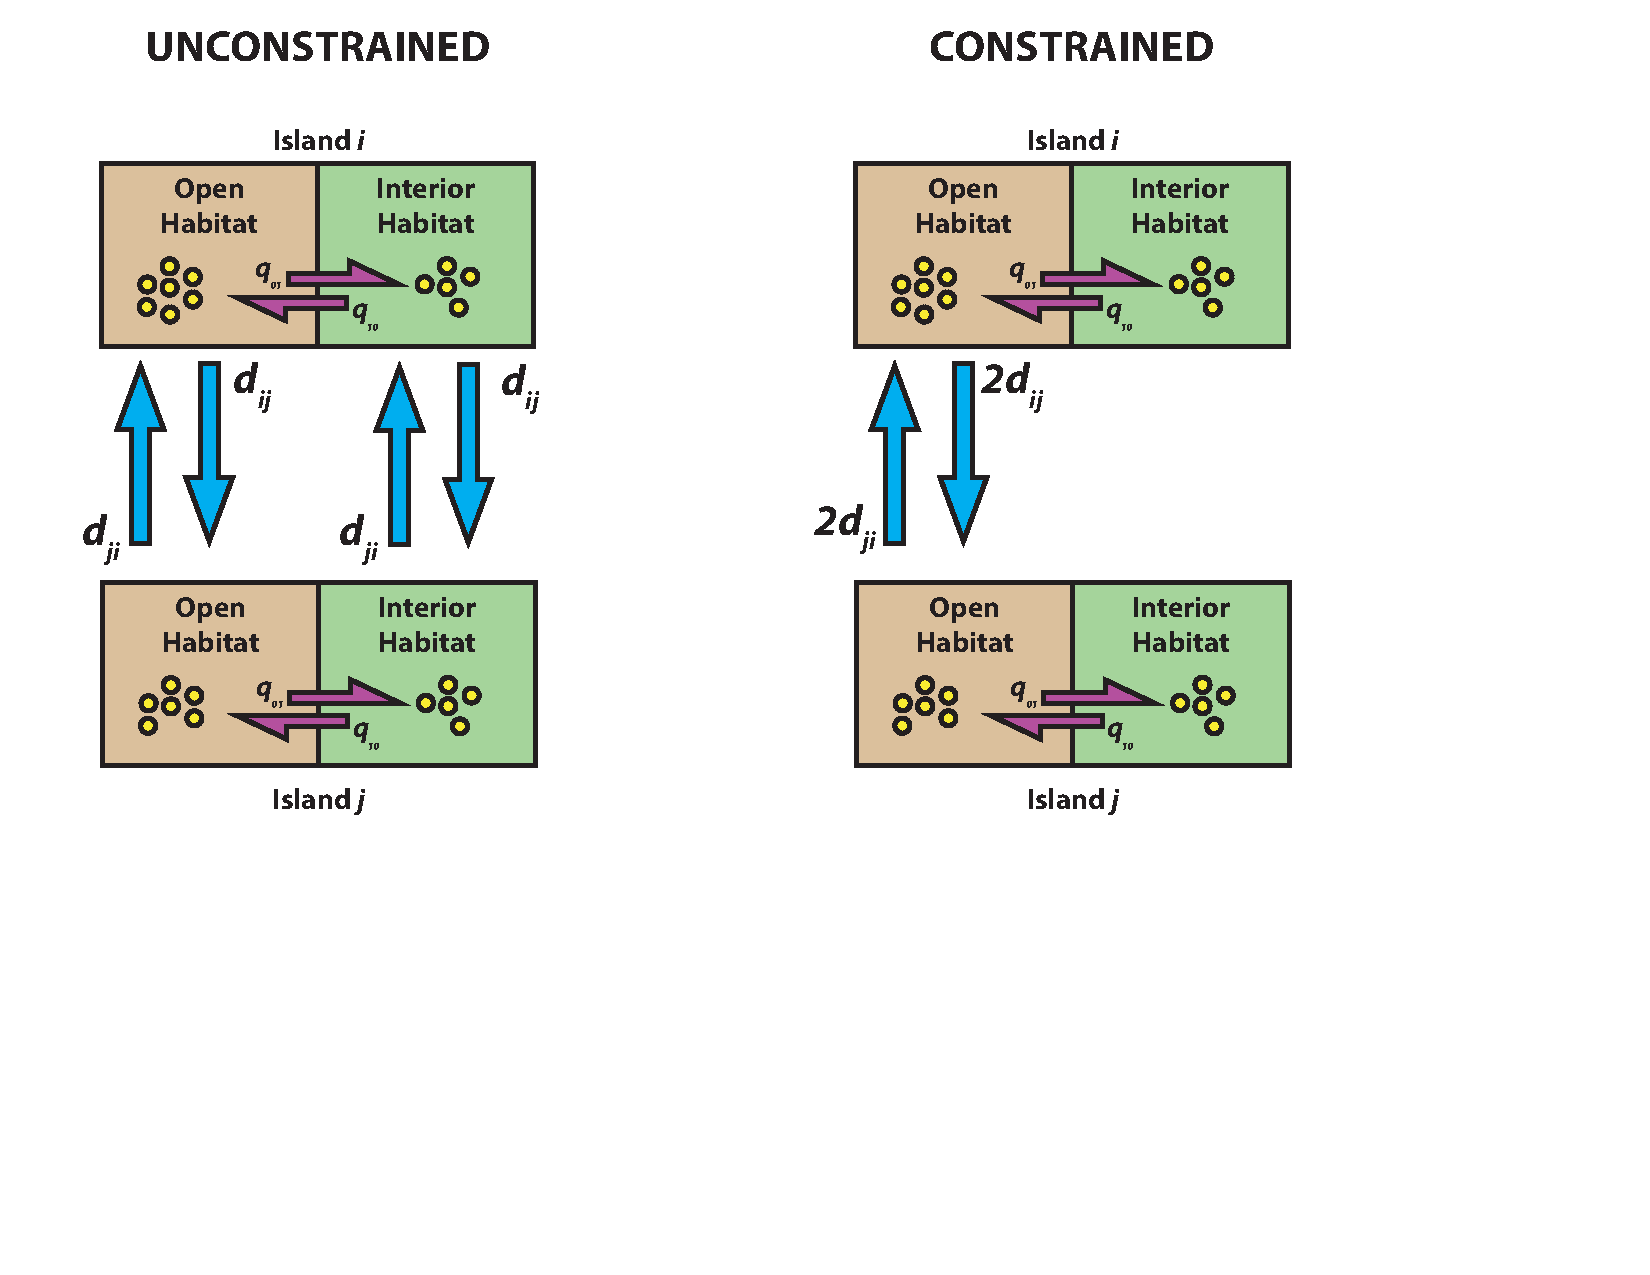
\includegraphics[scale=0.30]{figs/Experimental-Design-1.pdf}
        % \caption{default}
        % \label{fig:default}
    \end{center}
  \vspace{-80pt}
% \end{figure}
\end{wrapfigure}

As an example of a very basic analysis, let us consider testing whether or not dispersal is constrained by habitat association of a lineage (Figure).
We propose two different models, each corresponding to a different dispersal regime.
In the ``unconstrained'' model, lineages are free to disperse between islands regardless of their habitat affinities.
In the ``constrained'' model, ony lineages associated with the disturbed or open habitats can disperse between islands, while lineages associated with interior habitats are not able to disperse.
The habitat affinities of the lineages themselves are modeled as a discrete binary trait that evolves stochasitcally over the phylogeny.
That is, each lineage has a habitat trait, which can either be in the ``disturbed'' or ``interior'' state, and the state of this trait determines whether or not the lineage is capable of dispersing in the ``constrained'' model.
Thus, in the unconstrained model, lineages disperse between interior habitats on different islands directly.
In the constrained model, on the other hand, lineages cannot disperse between interior habitats directly: they have to move into a disturbed habitat association in ecological space over evolutionary time, at which phase they are capable of dispersing into new islands, and then re-invade the interior habitats on those new islands by, again, moving into them in ecological space over evolutionary time.
%%%%% EXAMPLE %%%%%%





%%%%% EXAMPLE %%%%%%

\end{document}
